\documentclass[11pt]{article}
\usepackage[margin=1.05in]{geometry}
\usepackage[T1]{fontenc}
\usepackage[utf8]{inputenc}
\usepackage{lmodern}
\usepackage{amsmath,amssymb,amsthm}
\usepackage{booktabs,array,longtable}
\usepackage{graphicx}
\usepackage{microtype}
\usepackage{tikz}
\usetikzlibrary{arrows.meta,positioning,calc}
\usepackage[colorlinks=true,allcolors=black,linkcolor=black,citecolor=black,
            urlcolor=blue]{hyperref}

\theoremstyle{plain}
\newtheorem{theorem}{Theorem}[section]
\newtheorem{proposition}[theorem]{Proposition}
\newtheorem{lemma}[theorem]{Lemma}
\newtheorem{corollary}[theorem]{Corollary}
\theoremstyle{definition}
\newtheorem{definition}[theorem]{Definition}
\newtheorem{example}[theorem]{Example}
\theoremstyle{remark}
\newtheorem{remark}[theorem]{Remark}

\newcommand{\pos}[1]{\left[#1\right]_{+}}
\newcommand{\mumol}{\ensuremath{\mu\mathrm{mol}}}
\newcommand{\R}{\mathbb{R}}
\newcommand{\leanref}[1]{{\normalfont\sffamily\footnotesize[\,#1\,]}}
\newcommand{\Lc}{L}

\title{\bfseries Certifying fresh microbial conversion from finite challenge
records: a sharp two-pool material bound}

\author{}
\date{17 September 2026}

\begin{document}
\maketitle

\begin{abstract}
A finite record of product collected from a microbial preparation is
compatible both with fresh conversion and with release of material that was
already present. We study this ambiguity in a two-window material model with
a mobile product pool, a convertible reserve pool, release, uptake, losses,
and an intervening recovery step with pool-specific retention. Given
calibrated upper bounds on initial stock $B$, on the pre-wash reserve $J$,
on credited recovery input $H$, and retention factors $0\le e\le s\le1$, we
prove that the fresh credited inventory $F_1+F_2$ generated during the two
windows is at least $\Lc$, the maximum of five affine expressions in the two
observed collections, and that $\Lc$ is \emph{exactly} the minimum of
$F_1+F_2$ over the declared class: an explicit finite material schedule
attains it from every admissible initial split of the stock. The lower
bound, an equivalent remaining-stock form, the attaining schedule and the
resulting exactness statement are verified in Lean~4 against Mathlib.
An exact counterexample shows that an initial reserve ceiling cannot be
substituted for the pre-wash ceiling, because uptake during the first window
moves mobile product into the better retained pool; we also verify a
zero-fresh history lying inside the reported output envelopes of our worked
record. We then prove that a bound on the initial reserve together with a
cumulative uptake cap is a valid alternative premise: the same five
expressions, evaluated at $J_0=\overline R+\overline T$, remain sound and
remain exactly attained, so destructive pre-wash measurement is sufficient
but not necessary.
Finally we quantify what a wash buys. At a matched material source the
mobile retention factor cancels from the certificate, so removing known
product is not itself an improvement; the entire benefit is attenuation of
first-window measurement uncertainty, worth $(s-e)\bigl(\epsilon_1-(J-r)\bigr)$
in the regime where the reserve-sensitive expression is active. In a
synthetic $10\,$mL example the washed certificate is $1.69$ \mumol\ against
$1.52$ \mumol\ for a matched unwashed protocol, and that $0.17$ \mumol\
margin is erased by reserve slack $\delta$ or by lost productive activity:
strict improvement holds exactly when the retained activity exceeds
$\tfrac{193}{210}+\tfrac{17}{42}\delta$. All numerical inputs are synthetic.
The results are an assay-design theory with a proposed biological
application; they are not biologically calibrated, and the certificate does
not assert substrate-specific atom attribution, viability, or future
function.
\end{abstract}

\noindent\textbf{Keywords.} exact lower certificate; material balance;
weak duality; assay design; identifiability; formal verification.

\medskip
\noindent\textbf{MSC 2020.} 90C05, 92C42, 68V20, 62P10.

\tableofcontents

\section{Introduction}

\subsection{The decision a challenge record is asked to support}

A common experiment presents a microbial preparation with a substrate,
collects product after a fixed window, intervenes---washes, dilutes,
resuspends---and then collects product again. The question the experiment is
meant to answer is whether the preparation \emph{converted} anything: whether
the collected product forces the conclusion that new material entered the
credited inventory during the observed windows.

The record does not answer this by itself. Product can be exported because it
was made, or because it was already present in the vessel, inside cells, on
surfaces, or in the medium, and was merely mobilised. Worse, the two
explanations are not separated by collecting more product: a preparation that
stores mobile product during the first window arrives at the intervention with
\emph{more} explanatory material than it started with, precisely in the
compartment that an intervention is least able to remove.

This paper isolates that ambiguity and answers it completely, in a
deliberately small model. We fix a two-pool material accounting, declare which
calibration bounds an experimenter is willing to supply, and compute the exact
minimum of the fresh amount over every material history compatible with the
record and those bounds. The answer is a maximum of five affine expressions.
Because it is a minimum and not merely a bound, it simultaneously certifies
what the record forces and identifies the information barrier: no sharper
certificate exists under the same premises, and improving the result requires
naming an additional measurement or a valid mechanistic restriction that
excludes the extremal schedule.

\subsection{Contributions}

\begin{enumerate}
\item \textbf{An exact certificate} (\S\ref{sec:certificate}). For a finite
two-window material source with mobile product, convertible reserves,
release, uptake, arbitrary losses and pool-specific recovery, the fresh
credited inventory satisfies $F_1+F_2\ge \Lc$, where $\Lc$ is the maximum of
five affine expressions in the observed collections
(Theorem~\ref{thm:sound}). An equivalent remaining-stock form
(Proposition~\ref{prop:closed}) exposes the mechanism: $\Lc$ is the
first-window deficit plus whatever second-window output cannot be explained
by optimally placing the leftover stock in the better retained pool.

\item \textbf{Exactness, formally verified} (\S\ref{sec:attain}). An explicit
finite schedule attains $\Lc$, starting from \emph{any} admissible split of
the initial stock between the two pools (Theorem~\ref{thm:attain}), so $\Lc$
is the least element of the set of achievable fresh totals
(Corollary~\ref{cor:least}). The attainment argument is machine-checked, not
only the inequality.

\item \textbf{The reserve premise: necessity and a substitute}
(\S\ref{sec:reserve}). A verified counterexample shows that the initial
reserve ceiling cannot be substituted for the pre-wash ceiling: a history
with zero fresh conversion receives a false certificate of $1.7$ \mumol\
(Theorem~\ref{thm:storage}). Nevertheless direct destructive reserve
measurement is \emph{not} mathematically mandatory. We prove that a bound on
the initial reserve together with a cumulative uptake cap gives a sound
certificate with $J_0=\overline R+\overline T$ (Theorem~\ref{thm:uptake}),
and that the resulting expression is again exactly attained
(Theorem~\ref{thm:uptakeattain}). Three of the five expressions use no
reserve information at all, so positive certification is sometimes possible
with none.

\item \textbf{What a wash can and cannot buy} (\S\ref{sec:wash}). At a matched
material source the mobile retention factor cancels from the certificate:
removing known product removes it from the explanatory background and from
the observed output in equal measure. The residual benefit is attenuation of
first-window measurement uncertainty, and it is exactly
$(s-e)\bigl(\epsilon_1-(J-r)\bigr)$ in the relevant regime, so reserve slack
alone can consume it. In the worked synthetic example we compute the full
joint budget in exact arithmetic: with reserve slack $\delta\ge0$ and
retained productive activity $a\in[0,1]$, washing strictly improves the
certificate if and only if $a>\tfrac{193}{210}+\tfrac{17}{42}\delta$
(Theorem~\ref{thm:budget}), which is already infeasible at $\delta=0.2$.

\item \textbf{A stated evidence boundary} (\S\ref{sec:evidence}). We separate
machine-checked statements, conventional arguments, exact computations and
unvalidated empirical premises, and we say which is which for every claim.
\end{enumerate}

\subsection{What is not claimed}\label{sec:notclaimed}

The target is \emph{fresh credited inventory}: material that entered a
declared, conservatively bounded pool during the two windows. That is a
weaker and more defensible object than ``de novo production'' of a named
molecule. In particular a certificate $F_1+F_2\ge\Lc>0$ does not establish
gross product-only formation if fresh material may enter convertible
intermediates; it does not attribute carbon atoms to a particular substrate;
it does not certify viability, growth, abundance or a per-cell rate; it does
not certify recovery relative to a demonstrably positive first window; and it
says nothing about function after the second window. Each of these is a
different target requiring its own observation or biological bridge. A zero
certificate is an \emph{unresolved} outcome---a statement about available
information---and never a certificate of death or of absent capability.

The numerical example throughout is synthetic. No biological calibration of
$B$, $J$, $e$, $s$, $H$, $\epsilon_k$ or the activity parameter $a$ has been
performed, and the percentages we compute are properties of a declared
response model, not measured properties of any wash technique or strain.

\subsection{Related work}

Absolute microbial load carries information that compositional profiling does
not~\cite{vandeputte}, but it supplies no reserve-per-cell calibration.
Dynamic metabolic flux analysis infers fluxes from transient concentration
records together with observability and reconciliation
analysis~\cite{leighty}, and recent enzyme-constrained variants propagate
uncertainty by bootstrapping~\cite{pennington}. We claim neither
uncertainty-aware flux inference nor exact linear programming as new. Our
contribution is narrower and of a different type: an exact minimum, with its
attaining history, for a small material class under explicitly declared
calibration bounds. \S\ref{sec:kinetic} states the precise relationship: a
\emph{valid} kinetic restriction shrinks the admissible class and can only
strengthen a lower certificate, so the comparison is about assumption
dependence rather than about method superiority.

For biological motivation we rely on defined-culture cross-feeding
studies~\cite{belenguer} and on strain-resolved lactate
utilisation~\cite{duncan,munoz}; \S\ref{sec:pilot} explains why a direct
lactate challenge tests a downstream conversion rather than a complete
community process, and corrects a natural but unsupported choice of reference
organism.

\subsection{Organisation}
\S\ref{sec:model} fixes the material model and the accounting boundary.
\S\ref{sec:certificate} proves the certificate and its closed form,
\S\ref{sec:attain} its exactness. \S\ref{sec:reserve} treats the reserve
premise, its necessity and its substitute. \S\ref{sec:noise} is the
observation wrapper and reporting rule. \S\ref{sec:wash} is the design
analysis. \S\ref{sec:evidence} states the evidence boundary,
\S\ref{sec:pilot} the calibration requirements and a feasibility pilot, and
\S\ref{sec:disc} the limitations. Appendix~\ref{app:repro} lists the source
modules, receipts and reproduction commands.

\section{The material model}\label{sec:model}

\subsection{Pools, units and the accounting boundary}

Fix one experimental unit: a single cultured aliquot with a preparation
identifier. \emph{All} amounts are referred to that original aliquot, never to
retained volume and never to surviving cells.

Two pools are tracked.
\begin{itemize}
\item $P$, \emph{mobile extracellular product}: the amount physically
available for collection.
\item $R$, \emph{convertible reserves}: everything else in the declared system
capable of contributing to credited output. This must include intracellular
intermediates, mobilisable biomass carbon, sorbed product and relevant
alternative nutrients, each entered at a conservative product-equivalent upper
yield.
\end{itemize}

The credited inventory is measured in product equivalents; in the worked
example, \mumol\ of butyrate equivalents, one equivalent per four creditable
carbon atoms. Declaring a pool inert because it is inconvenient is not a
calibration, and conversely a conservative carbon potential may be much larger
than the measured product, which makes $B$ large and the certificate weak.
That is an informative limitation of the assay, not a defect of the theorem.

Two conventions must be fixed before any calculation.

\begin{enumerate}
\item \emph{The position of unreacted challenge substrate.} If it lies outside
the credited pools, then the event counted as fresh conversion is exactly its
movement into them. It cannot simultaneously be charged as old explanatory
stock and counted again as a new positive source. A complete implementation
should list every carbon-bearing input and assign it to initial stock, fresh
conversion, recovery input, or another explicitly bounded source.
\item \emph{Collection versus retention.} $Q_k$ is material that physically
leaves the boundary in window $k$, and the two windows are nonoverlapping. A
retained endpoint pool is not also counted as exported. For a homogeneous
sample of volume $v$ from volume $V$ at concentration $c$,
\[
 Vc=(V-v)c+vc ,
\]
the second term is counted once as collected and the first is carried forward
with its state. Wash waste is excluded from $Q_1,Q_2$ in the protocol declared
here and may be reported separately.
\end{enumerate}

\begin{figure}[t]
\centering
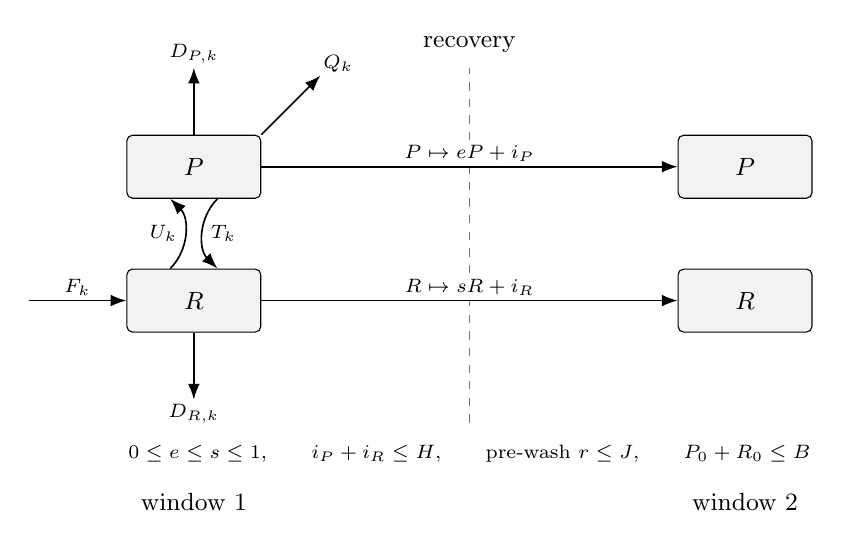
\begin{tikzpicture}[
  pool/.style={draw,rounded corners=2pt,minimum width=1.7cm,
               minimum height=0.8cm,font=\small,fill=black!5},
  ev/.style={-{Latex[length=2mm]},semithick},
  lab/.style={font=\scriptsize,inner sep=1.5pt}]

  \node[pool] (P1) at (0,1.7) {$P$};
  \node[pool] (R1) at (0,0)   {$R$};
  \node[pool] (P2) at (7.0,1.7) {$P$};
  \node[pool] (R2) at (7.0,0)   {$R$};

  % internal transfers in window 1
  \draw[ev] ($(R1.north)+(-0.3,0)$) to[bend right=45]
     node[lab,left=1pt]{$U_k$} ($(P1.south)+(-0.3,0)$);
  \draw[ev] ($(P1.south)+(0.3,0)$) to[bend right=45]
     node[lab,right=1pt]{$T_k$} ($(R1.north)+(0.3,0)$);

  % boundary events
  \draw[ev] (-2.1,0) -- (R1.west) node[lab,above,midway]{$F_k$};
  \draw[ev] (P1.north) -- ++(0,0.85) node[lab,above]{$D_{P,k}$};
  \draw[ev] (R1.south) -- ++(0,-0.85) node[lab,below]{$D_{R,k}$};
  \draw[ev] (P1.north east) -- ++(0.75,0.75)
     node[lab,above right=-1pt]{$Q_k$};

  % recovery
  \draw[dashed,black!55] (3.5,-1.55) -- (3.5,2.95);
  \node[font=\small] at (3.5,3.25) {recovery};
  \draw[ev] (P1.east) -- (P2.west)
     node[lab,above,midway,fill=white]{$P\mapsto eP+i_P$};
  \draw[ev] (R1.east) -- (R2.west)
     node[lab,above,midway,fill=white]{$R\mapsto sR+i_R$};

  \node[font=\scriptsize] at (3.5,-1.95)
    {$0\le e\le s\le 1$,\qquad $i_P+i_R\le H$,\qquad
     pre-wash $r\le J$,\qquad $P_0+R_0\le B$};
  \node[font=\small] at (0,-2.55) {window 1};
  \node[font=\small] at (7.0,-2.55) {window 2};
\end{tikzpicture}
\caption{The declared accounts. Arrows are material transfers in a finite
schedule, not fitted kinetics. Productive activity is not a material pool;
its retention is a separate calibration and does not follow from $e$ or $s$.}
\label{fig:protocol}
\end{figure}

\subsection{Finite source histories}

\begin{definition}[Window]\label{def:window}
A \emph{window} is a tuple
$w=(p_0,r_0,F,U,T,Q,D_P,D_R)\in\R^8$ of nonnegative reals satisfying the
availability constraints
\begin{equation}
 U\le r_0+F,\qquad
 U+D_R\le r_0+F+T,\qquad
 T+Q+D_P\le p_0+U ,
 \label{eq:avail}
\end{equation}
with terminal pools
\begin{equation}
 p(w)=p_0+U-T-Q-D_P,\qquad
 r(w)=r_0+F+T-U-D_R .
 \label{eq:update}
\end{equation}
Here $F$ is fresh credited conversion, $U$ release from reserve into mobile
product, $T$ uptake or storage from mobile product into reserve, $Q$
collection, and $D_P,D_R$ are unrestricted loss accounts.
\end{definition}

Constraints~\eqref{eq:avail} implement a definite event order---fresh
addition, release, uptake, collection, loss---with enough material present at
each step. A window is therefore an actual nonnegative schedule, not merely an
assumed inequality between observables.

\begin{lemma}[Pool nonnegativity and balance]\label{lem:balance}
\leanref{pool\_nonneg, source\_balance}
For every window $w$, $p(w)\ge0$ and $r(w)\ge0$, and
\begin{equation}
 Q+p(w)+r(w)+D_P+D_R=p_0+r_0+F .
 \label{eq:bal}
\end{equation}
Consequently $Q+p(w)+r(w)\le p_0+r_0+F$.
\end{lemma}

\begin{proof}
Nonnegativity is immediate from~\eqref{eq:avail} and~\eqref{eq:update}:
$p(w)=(p_0+U)-(T+Q+D_P)\ge0$ and
$r(w)=(r_0+F+T)-(U+D_R)\ge0$. Identity~\eqref{eq:bal} is the sum
of the two lines of~\eqref{eq:update}, in which $U$ and $T$ cancel. The
inequality follows from $D_P,D_R\ge0$.
\end{proof}

Equation~\eqref{eq:bal} is why release, uptake and losses need never be
identified individually: they cancel or are dropped in one direction. The
same summed identity holds for any finer admissible interleaving that
respects the same pool availability, though only the displayed finite source
is formalised.

\begin{definition}[History]\label{def:history}
A \emph{history} is a pair of windows $w_1,w_2$ together with retention
factors $0\le e\le s\le 1$ and nonnegative recovery inputs $i_P,i_R$ obeying
\begin{equation}
 (w_2)_{p_0}\le e\,p(w_1)+i_P,
 \qquad
 (w_2)_{r_0}\le s\,r(w_1)+i_R .
 \label{eq:recovery}
\end{equation}
\end{definition}

We write $p=p(w_1)$, $r=r(w_1)$ for the latent pre-recovery state,
$F_1,F_2$ for the two fresh amounts and $Q_1,Q_2$ for the two collections.
The factors $e$ and $s$ are \emph{calibrated upper retention maps} for the two
pools, obtained by measuring recovery of the relevant analyte through the
actual intervention. A dilution factor is not automatically a process
recovery, $s$ does not follow from $e$, and neither of them bounds retained
productive activity, which is a separate parameter and is never inferred from
a material retention factor.

\begin{lemma}[Recovery account]\label{lem:recov}
\leanref{recovery\_account}
For every history,
$Q_2\le e\,p+s\,r+i_P+i_R+F_2$.
\end{lemma}

\begin{proof}
By Lemma~\ref{lem:balance} applied to $w_2$,
$Q_2\le (w_2)_{p_0}+(w_2)_{r_0}+F_2$, and~\eqref{eq:recovery} bounds the two
initial pools.
\end{proof}

\subsection{Calibration data and observations}

The certificate consumes the following, each of which must be an upper bound
valid on the same event:
\[
 P_0+R_0\le B,\qquad
 r\le J,\qquad
 i_P+i_R\le H,\qquad
 0\le e\le s\le 1,
\]
together with lower bounds $q_1\le Q_1$, $q_2\le Q_2$ on the two collections.
Section~\ref{sec:noise} explains how $q_k$ is produced from a reported value
and an error allowance. $J$ bounds the reserve \emph{immediately before
recovery}; \S\ref{sec:reserve} shows that this is not the same as a bound on
the initial reserve, and gives an alternative premise that avoids measuring it
directly.

\subsection{A stoichiometric witness}

For the lactate/acetate application the net conversion
\begin{equation}
 4\,\mathrm{C_3H_6O_3}+2\,\mathrm{C_2H_4O_2}
 \longrightarrow
 3\,\mathrm{C_4H_8O_2}+4\,\mathrm{CO_2}+2\,\mathrm{H_2}+2\,\mathrm{H_2O}
 \label{eq:chem}
\end{equation}
balances carbon, hydrogen and oxygen \leanref{balanced\_conversion}. This is
an accounting witness that a net material conversion is possible. It is not a
rate, a thermodynamic feasibility statement for a chosen medium, an
organism-specific pathway, or an atom mapping. The mathematical source admits
loss to competing products; any further positive source must enter the initial
stock or the recovery account.

\section{The exact certificate}\label{sec:certificate}

Throughout, $\pos{z}=\max(0,z)$.

\begin{definition}\label{def:L}
For $q_1,q_2,B,e,s,J,H\in\R$ put
\begin{equation}
 \Lc(q_1,q_2;B,e,s,J,H)=\max\left\{
 \begin{aligned}
 &0,\\
 &q_1-B,\\
 &q_1+q_2-B-H,\\
 &e q_1+q_2-eB-(s-e)J-H,\\
 &s q_1+q_2-sB-H
 \end{aligned}\right\} .
 \label{eq:facets}
\end{equation}
\end{definition}

We refer to the five entries as the \emph{nonnegativity}, \emph{first-window},
\emph{total}, \emph{reserve-sensitive} and \emph{uniform-retention}
expressions. They are a maximum of five affine lower bounds, not five
irredundant facets in every parameter slice: at $e=s$ the reserve-sensitive
entry is dominated by the uniform one, and other coincidences occur at
degenerate parameters.

\subsection{Soundness}

\begin{theorem}[Source-bound certificate]\label{thm:sound}
\leanref{lower\_sound, observed\_source\_bound}
Let a history satisfy $P_0+R_0\le B$, $r\le J$, $i_P+i_R\le H$, and let
$q_1\le Q_1$, $q_2\le Q_2$. Then
\[
 F_1+F_2\ \ge\ \Lc(q_1,q_2;B,e,s,J,H).
\]
\end{theorem}

\begin{proof}
Lemma~\ref{lem:balance} applied to $w_1$ and the stock bound give
\begin{equation}
 q_1+p+r\ \le\ Q_1+p+r\ \le\ P_0+R_0+F_1\ \le\ B+F_1 ,
 \label{eq:acc1}
\end{equation}
and Lemma~\ref{lem:recov} with the input bound gives
\begin{equation}
 q_2\ \le\ Q_2\ \le\ e\,p+s\,r+H+F_2 .
 \label{eq:acc2}
\end{equation}
We produce each entry of~\eqref{eq:facets} as a nonnegative combination
of~\eqref{eq:acc1}, \eqref{eq:acc2} and $r\le J$.

\emph{Nonnegativity.} $F_1+F_2\ge0$ because fresh amounts are nonnegative.

\emph{First-window.} From~\eqref{eq:acc1} and $p,r\ge0$, $q_1-B\le F_1\le
F_1+F_2$.

\emph{Total.} Add~\eqref{eq:acc1} and~\eqref{eq:acc2}. Since $e\le 1$ and
$s\le1$ we have $ep+sr\le p+r$, so
\[
 q_1+q_2\le B+H+F_1+F_2-(1-e)p-(1-s)r\le B+H+F_1+F_2 .
\]

\emph{Reserve-sensitive.} Multiply~\eqref{eq:acc1} by $e\ge0$ and
add~\eqref{eq:acc2}, writing $ep+sr=e(p+r)+(s-e)r$:
\[
 e q_1+q_2\le e B+eF_1+(s-e)r+H+F_2
 \le eB+(s-e)J+H+F_1+F_2 ,
\]
using $r\le J$, $s\ge e$ and $eF_1\le F_1$.

\emph{Uniform-retention.} Multiply~\eqref{eq:acc1} by $s\ge0$ instead and use
$ep\le sp$:
\[
 s q_1+q_2\le sB+sF_1+H+F_2-(s-e)p\le sB+H+F_1+F_2 .
\]
Taking the maximum of the five conclusions proves the theorem.
\end{proof}

These are explicit weak-duality certificates: fixed nonnegative multipliers
applied to material constraints. No linear-programming solver is invoked at
run time, and nothing here should be described as a verified general
LP-duality engine.

\subsection{The remaining-stock form}

\begin{proposition}[Closed form]\label{prop:closed}
\leanref{lower\_closed}
Let $0\le e\le s\le 1$ and $J\ge0$. With
\[
 A=\pos{q_1-B},\qquad x=\pos{B-q_1},\qquad
 K(x)=e\,x+(s-e)\min(J,x),
\]
one has, for all $q_1,q_2,B,H\in\R$,
\begin{equation}
 \Lc(q_1,q_2;B,e,s,J,H)=A+\pos{q_2-H-K(x)} .
 \label{eq:closed}
\end{equation}
\end{proposition}

\begin{proof}
Note $A-x=q_1-B$ and $A\,x=0$.

\emph{($\le$).} Write $M=A+\pos{q_2-H-K(x)}$. Since $s\le1$ and
$\min(J,x)\le x$,
\[
 K(x)\le e x+(s-e)x=sx\le x,
 \qquad
 K(x)\le ex+(s-e)J .
\]
Both summands of $M$ are nonnegative, so the entry $0$ satisfies $0\le M$, and
$q_1-B=A-x\le A\le M$. For the remaining three entries, using $eA\le A$ and
$sA\le A$,
\begin{align*}
 q_1+q_2-B-H &= A+\bigl(q_2-H-x\bigr), \\
 e q_1+q_2-eB-(s-e)J-H &= eA+\bigl(q_2-H-ex-(s-e)J\bigr), \\
 s q_1+q_2-sB-H &= sA+\bigl(q_2-H-sx\bigr),
\end{align*}
and in each case the bracket is at most $q_2-H-K(x)\le\pos{q_2-H-K(x)}$, so
each left-hand side is at most $M$.

\emph{($\ge$).} If $q_1\le B$ then $A=0$ and $x=B-q_1$. When $x\le J$,
$K(x)=sx$ and $A+\pos{q_2-H-K(x)}=\max\{0,\,s q_1+q_2-sB-H\}$, a maximum of
two entries of~\eqref{eq:facets}. When $x\ge J$, $K(x)=ex+(s-e)J$ and the
expression equals $\max\{0,\,e q_1+q_2-eB-(s-e)J-H\}$, again a maximum of two
entries. If $q_1\ge B$ then $x=0$, $K(0)=0$ and the expression equals
$(q_1-B)+\pos{q_2-H}=\max\{q_1-B,\;q_1+q_2-B-H\}$.
In every case the right-hand side of~\eqref{eq:closed} is a maximum of entries
of~\eqref{eq:facets}, hence at most $\Lc$.
\end{proof}

Form~\eqref{eq:closed} is the mechanism behind the formula. $A$ is
first-window formation that cannot be avoided. The credited stock still
available after the first collection is $x$. To explain as much of the second
collection as possible an adversary places up to $J$ of that remainder in the
better retained reserve pool and the rest in the mobile pool, producing
maximal explanatory carryover $K(x)$. Fresh conversion is forced only by the
part of $q_2$ that survives $H$ and $K(x)$.

\begin{remark}[Scalar specialisation]
At $e=s=\rho$ the reserve information is inert, $K(x)=\rho x$, and
\eqref{eq:closed} becomes $\pos{q_1-B}+\pos{q_2-H-\rho\pos{B-q_1}}$. This
single-pool formula is inherited background for the present work and is not
claimed as a discovery here; the two-pool refinement is what requires the
pre-wash reserve bound.
\end{remark}

\begin{remark}[Endpoints]
No step divides by a retention factor, so $e=0$, $s=0$, $e=s=1$, $B=0$, $H=0$
and all equality boundaries are included.
\end{remark}

\subsection{Monotonicity and sensitivity}

The following consequences of~\eqref{eq:closed} are what an interface should
report instead of a fixed narrative about which measurement to improve.

\begin{proposition}[Sensitivity]\label{prop:sens}
Fix $0\le e\le s\le1$ and $B,H$. Then $\Lc$ is nondecreasing in $q_1$ and
$q_2$, nonincreasing in $B$, $H$ and $J$, and:
\begin{enumerate}
\item[(i)] $\Lc$ does not depend on $J$ once $J\ge x=\pos{B-q_1}$; in
particular tightening a reserve bound above the remaining stock buys nothing.
\item[(ii)] For $0\le J\le J'\le x$,
$\;0\le \Lc(J)-\Lc(J')\le (s-e)(J'-J)$, with equality when both second
brackets in~\eqref{eq:closed} are positive.
\item[(iii)] If $e=s$ then $\Lc$ does not depend on $J$ at all.
\end{enumerate}
\end{proposition}

\begin{proof}
Monotonicity in $q_1,q_2,B,H$ is entry-wise in~\eqref{eq:facets}, all
coefficients of $q_1$ being $0,1,1,e,s\ge0$. For the rest use
\eqref{eq:closed}: $J\mapsto K(x)=ex+(s-e)\min(J,x)$ is nondecreasing, is
constant for $J\ge x$, and increases by exactly $(s-e)(J'-J)$ on $[0,x]$;
$\pos{\cdot}$ is nondecreasing and $1$-Lipschitz. Part~(iii) is $s-e=0$.
\end{proof}

\section{Exactness}\label{sec:attain}

Theorem~\ref{thm:sound} would be of limited value if it were not tight: an
experimenter needs to know whether an unresolved record reflects a weak
argument or a genuine information barrier. It is tight, and the attaining
schedule is explicit.

\begin{theorem}[Attainment]\label{thm:attain}
\leanref{lower\_attained}
Let $q_1,q_2,B,J,H\ge0$ and $0\le e\le s\le1$, and let $R_0\in[0,B]$ be any
initial reserve level. Then there is a history with
\[
 P_0=B-R_0,\quad R_0=R_0,\quad Q_1=q_1,\quad Q_2=q_2,\quad
 r\le J,\quad i_P+i_R\le H,
\]
whose first-window uptake satisfies $T_1\le\pos{\min(J,B)-R_0}$ and whose
fresh total is exactly
\[
 F_1+F_2=\Lc(q_1,q_2;B,e,s,J,H).
\]
\end{theorem}

\begin{proof}
Write $A=\pos{q_1-B}$, $x=\pos{B-q_1}$, $r=\min(J,x)$ and $p=x-r\ge0$. Set
\[
 F_1=A,\qquad U_1=\pos{R_0+A-r},\qquad T_1=\pos{r-R_0-A},
 \qquad Q_1=q_1,
\]
with $D_{P,1}=D_{R,1}=0$. At most one of $U_1,T_1$ is positive and
$U_1-T_1=R_0+A-r$. Consequently
\[
 r(w_1)=R_0+A+T_1-U_1=r,\qquad
 p(w_1)=(B-R_0)+U_1-T_1-q_1=B+A-q_1-r=x-r=p ,
\]
using $A-x=q_1-B$. The three availability
constraints~\eqref{eq:avail} for $w_1$ are exactly $U_1\le R_0+A$ (true since
$U_1=\pos{R_0+A-r}$ and $R_0+A\ge0$), $r(w_1)\ge0$ and $p(w_1)\ge0$, all of
which hold. Also $r\le J$ and $r\le x\le B$, so
$T_1=\pos{r-R_0-A}\le\pos{\min(J,B)-R_0}$.

For the recovery step take $i_P=0$, $i_R=H$, so
$(w_2)_{p_0}=e\,p$ and $(w_2)_{r_0}=s\,r+H$, which satisfy~\eqref{eq:recovery}
with equality. Since $p+r=x$ and $r=\min(J,x)$,
\[
 e\,p+s\,r=e\,x+(s-e)\,r=K(x).
\]
Now set
\[
 F_2=\pos{q_2-H-K(x)},\qquad
 U_2=\pos{q_2-e\,p},\qquad T_2=0,\qquad Q_2=q_2,
\]
\[
 D_{P,2}=e\,p+U_2-q_2\ \ge 0,\qquad
 D_{R,2}=s\,r+H+F_2-U_2\ \ge 0 .
\]
Nonnegativity of $D_{P,2}$ is $U_2\ge q_2-ep$. For $D_{R,2}$, both
$0\le sr+H+F_2$ and $q_2-ep\le sr+H+F_2$ hold---the latter because
$F_2\ge q_2-H-ep-sr$---so $U_2=\max(0,q_2-ep)\le sr+H+F_2$; this same
inequality is the third availability constraint $U_2\le (w_2)_{r_0}+F_2$. The
remaining two constraints of~\eqref{eq:avail} for $w_2$ hold with equality by
the definition of $D_{P,2}$ and $D_{R,2}$.

Finally $F_1+F_2=A+\pos{q_2-H-K(x)}$, which equals $\Lc$ by
Proposition~\ref{prop:closed}.
\end{proof}

\begin{corollary}[$\Lc$ is the exact minimum]\label{cor:least}
\leanref{lower\_is\_minimum}
Under the hypotheses of Theorem~\ref{thm:attain}, $\Lc(q_1,q_2;B,e,s,J,H)$ is
the least element of
\[
 \Bigl\{F_1+F_2 \;:\; \text{histories with retention }(e,s),\;
 P_0+R_0\le B,\ Q_1\ge q_1,\ Q_2\ge q_2,\ r\le J,\ i_P+i_R\le H\Bigr\}.
\]
\end{corollary}

\begin{proof}
Membership is Theorem~\ref{thm:attain} with $R_0=0$; the lower-bound property
is Theorem~\ref{thm:sound}.
\end{proof}

\begin{remark}[What sharpness does and does not say]\label{rem:sharp}
Corollary~\ref{cor:least} is a statement about the declared class, whose
initial state is \emph{bounded} by $B$ and whose uncertainty bounds may vary
independently unless an explicit constraint links them. The construction is
therefore free to combine unfavourable extremes---maximal stock, maximal
recovery input, maximal reserve---that a more detailed model might forbid. It
does not show that a particular strain can execute the schedule in a given
number of minutes: there are no calibrated transfer rates in the class. If a
valid correlation or kinetic restriction excludes the extremiser, the lower
bound remains sound and may cease to be attained; that is an opportunity to
strengthen the result, and any claim of better performance must name the
restriction that does it (\S\ref{sec:kinetic}).
\end{remark}

\section{The reserve premise: necessity, ambiguity, and a substitute}
\label{sec:reserve}

\subsection{An initial reserve ceiling is not a pre-wash ceiling}

\begin{theorem}[Storage counterexample]\label{thm:storage}
\leanref{storage\_counterexample, initial\_reserve\_substitution\_unsound}
There is a history with
\[
 P_0=8,\quad R_0=2,\quad Q_1=6,\quad T_1=2,\quad
 F_1=F_2=0,\quad e=\tfrac1{20},\ s=\tfrac9{10},\ i_P=i_R=0,
\]
whose pre-wash state is $(p,r)=(0,4)$ and whose second collection is
$Q_2=\tfrac{18}5$. Substituting the initial reserve ceiling $2$ for $J$ in
\eqref{eq:facets} returns $\Lc=\tfrac{17}{10}$, whereas the true fresh total
is $0$. Evaluated at the correct pre-wash ceiling $J=4$ the formula returns
$0$.
\end{theorem}

\begin{proof}
Take $w_1=(8,2,0,0,2,6,0,0)$; the availability
constraints~\eqref{eq:avail} read $0\le2$, $0\le4$ and $2+6\le8$, and
\eqref{eq:update} gives $p=0$, $r=4$. Take
$w_2=(0,\tfrac{18}5,0,\tfrac{18}5,0,\tfrac{18}5,0,0)$; the recovery
inequalities~\eqref{eq:recovery} hold with equality since
$e\cdot0=0$ and $s\cdot4=\tfrac{18}5$. Both fresh amounts are zero. The two
evaluations of~\eqref{eq:facets} are arithmetic.
\end{proof}

The defect is storage of initially mobile product, not instrument noise,
numerical tolerance or insufficient proof effort. It refutes the
unconditional initial-reserve substitution. It does \emph{not} show that
destructive pre-wash measurement is the only repair, and it does not make $J$
necessary for every positive certificate: the nonnegativity, first-window,
total and uniform-retention entries of~\eqref{eq:facets} contain no reserve
information, so
\[
 \Lc\ \ge\ \max\{0,\ q_1-B,\ q_1+q_2-B-H,\ s q_1+q_2-sB-H\}
\]
is always available with no reserve calibration whatsoever, and is positive in
some regimes.

\subsection{The worked record does need it}

Necessity is nevertheless real for the example we use in \S\ref{sec:wash}.

\begin{theorem}[The reserve premise is not redundant there]
\label{thm:ambiguity}
\leanref{reserve\_premise\_not\_redundant}
There is a history with $P_0+R_0=10$, $i_P+i_R=\tfrac15$, retention
$e=\tfrac1{20}$, $s=\tfrac9{10}$, collections
$Q_1=\tfrac{29}5$ and $Q_2=\tfrac{381}{100}$---so
$|Q_1-6|\le\tfrac15$ and $|Q_2-4|\le\tfrac15$---pre-wash reserve $r=4$, and
$F_1+F_2=0$.
\end{theorem}

\begin{proof}
Take $w_1=(8,2,0,0,2,\tfrac{29}5,0,0)$, giving $p=\tfrac15$, $r=4$, and
$w_2=(\tfrac1{100},\tfrac{19}5,0,\tfrac{19}5,0,\tfrac{381}{100},0,0)$ with
$i_P=0$, $i_R=\tfrac15$. Then
$e\,p=\tfrac1{100}$ and $s\,r+i_R=\tfrac{18}5+\tfrac15=\tfrac{19}5$, so
\eqref{eq:recovery} holds with equality, and the availability constraints are
$\tfrac{19}5\le\tfrac{19}5$ and
$\tfrac{381}{100}\le\tfrac1{100}+\tfrac{19}5$.
\end{proof}

Both collections of this zero-fresh history lie inside the reported envelopes
of the positive witness of \S\ref{sec:wash}; the two differ only in the
pre-wash reserve, $4$ against $2$. The premise $r\le2$ excludes it; the two
product measurements alone do not (Figure~\ref{fig:ambiguity}). No claim is
made that the alternative also matches substrate, isotope or biomass
observations that were not part of the declared record---that is exactly the
kind of extra information that would strengthen the certificate.

\begin{figure}[t]
\centering

\includegraphics[width=0.86\linewidth]{figures/ambiguity.pdf}
\caption{Two exact material histories inside the same output envelopes. They
differ in the pre-wash reserve and in the fresh total. An independently
justified reserve ceiling separates them; the endpoint record does not.}
\label{fig:ambiguity}
\end{figure}

\subsection{Bounded uptake in place of direct reserve measurement}

Destructive measurement of the pre-wash reserve is expensive, consumes the
preparation, and needs its own transport and heterogeneity calibration. The
following shows it is sufficient but not necessary: a bound on the
\emph{initial} reserve together with a cap on \emph{cumulative first-window
uptake} supplies the same expression.

\begin{theorem}[Uptake-cap certificate]\label{thm:uptake}
\leanref{lower\_sound\_uptake, uptake\_source\_bound}
Let a history satisfy $P_0+R_0\le B$, $i_P+i_R\le H$, $q_1\le Q_1$,
$q_2\le Q_2$, and suppose valid bounds
\[
 R_0\le\overline R,\qquad T_1\le \overline T,\qquad
 J_0:=\overline R+\overline T .
\]
Then $F_1+F_2\ \ge\ \Lc(q_1,q_2;B,e,s,J_0,H)$.
\end{theorem}

\begin{proof}
From~\eqref{eq:update} and $U_1,D_{R,1}\ge0$
\leanref{prewash\_reserve\_from\_uptake},
\begin{equation}
 r=R_0+F_1+T_1-U_1-D_{R,1}\ \le\ J_0+F_1 .
 \label{eq:rbound}
\end{equation}
Note this is \emph{not} the claim $r\le J_0$, and that $F_1$ is unknown. The
four entries of~\eqref{eq:facets} that do not mention $J$ are unaffected, so
only the reserve-sensitive entry must be re-derived. Multiply
\eqref{eq:acc1} by $e$ and add~\eqref{eq:acc2}, writing
$ep+sr=e(p+r)+(s-e)r$ and using~\eqref{eq:rbound}:
\[
 q_2\le e\bigl(B+F_1-q_1\bigr)+(s-e)\bigl(J_0+F_1\bigr)+H+F_2
 = e(B-q_1)+(s-e)J_0+H+s F_1+F_2 .
\]
Since $s\le1$ and $F_1\ge0$, $sF_1\le F_1$, giving
$e q_1+q_2-eB-(s-e)J_0-H\le F_1+F_2$.
\end{proof}

The reason the unknown $F_1$ does no harm is precisely $s\le1$: material
formed during the first window and stored cannot have more than unit retained
explanatory value in the second. The bound is therefore not circular.

\begin{theorem}[Exactness under the uptake premise]\label{thm:uptakeattain}
\leanref{uptake\_bound\_attained}
Let $q_1,q_2,B,H,\overline R,\overline T\ge0$ and $0\le e\le s\le1$. There is
a history with $P_0+R_0\le B$, $Q_1=q_1$, $Q_2=q_2$, $R_0\le\overline R$,
$T_1\le\overline T$, $i_P+i_R\le H$ and
$F_1+F_2=\Lc(q_1,q_2;B,e,s,\overline R+\overline T,H)$.
\end{theorem}

\begin{proof}
Apply Theorem~\ref{thm:attain} with $J=J_0=\overline R+\overline T$ and
$R_0=\min(\overline R,B)$. Then $R_0\le\overline R$ and the theorem gives
$T_1\le\pos{\min(J_0,B)-R_0}$. If $\overline R\le B$ then $R_0=\overline R$
and $\min(J_0,B)-R_0\le J_0-\overline R=\overline T$; if $\overline R>B$ then
$R_0=B$ and $\min(J_0,B)-R_0\le0$. In both cases $T_1\le\overline T$.
\end{proof}

So the substitution $J:=\overline R+\overline T$ loses nothing: the same
expression is again the exact minimum, now over the uptake-bounded class.

\begin{remark}[How to obtain an uptake cap, and how it can fail]
A calibrated upper uptake rate yields a cumulative cap
$T_1\le\int_0^{h_1}v_{\max}X(t)\,dt\le v_{\max}X_{\max}h_1$ in consistent
product-equivalent units, which uses a mechanistic constraint without
requiring an identified kinetic model. Three cautions. The bound must be a
valid \emph{upper} rate for the preparation and conditions, not a best-fit
estimate. The cap concerns \emph{gross} uptake into the credited reserve, not
net extracellular disappearance: simultaneous release conceals uptake in a net
time course. And a cap on uptake of the wrong chemical species does not bound
storage of credited product.
\end{remark}

\begin{remark}[Combining the two premises]
If both a direct reserve bound $J$ and an uptake pair
$(\overline R,\overline T)$ are available and valid, compute both certificates
and report the maximum; both are sound. Keep the two premise records distinct.
In particular $J_0$ is not itself a proved bound on the actual pre-wash
reserve when $F_1>0$, and an interface documenting its input as a measured
pre-wash ceiling must not silently accept $J_0$ without recording the
different biological premise. On the history of Theorem~\ref{thm:storage} the
uptake route with $\overline R=\overline T=2$ gives $J_0=4$ and certifies
$0$, as it must \leanref{uptake\_route\_sound\_here}.
\end{remark}

\section{Observation uncertainty and the reporting rule}\label{sec:noise}

\subsection{A deterministic wrapper}

Let $y_k$ be reported output amounts with absolute allowances $\epsilon_k$,
and consider the simultaneous event
\[
 \mathcal E=\bigl\{\,|Q_1-y_1|\le\epsilon_1,\ |Q_2-y_2|\le\epsilon_2,\
 \text{and all stated calibration bounds hold}\,\bigr\}.
\]
On $\mathcal E$ put $q_k=\pos{y_k-\epsilon_k}$. Since $Q_k\ge0$ and
$Q_k\ge y_k-\epsilon_k$, these are valid lower bounds, and $\Lc$ is
nondecreasing in $q_1,q_2$ by Proposition~\ref{prop:sens}.

\begin{proposition}[Reporting guarantee]\label{prop:report}
\leanref{noisy\_observation, reporting, resolution}
On $\mathcal E$, issuing the verdict \emph{at or above} only when
$\Lc(q_1,q_2;B,e,s,J,H)\ge F_\star$ guarantees $F_1+F_2\ge F_\star$. If a
separately justified upper bound $U_F\ge F_1+F_2$ is supplied, issuing
\emph{below} only when $U_F<F_\star$ is likewise sound, and the record is
\emph{incompatible} when $\Lc>U_F$ or when some $y_k+\epsilon_k<0$. All other
records are \emph{unresolved}.
\end{proposition}

\begin{proof}
The first claim is Theorem~\ref{thm:sound} composed with transitivity; the
second is immediate. For incompatibility, $\Lc>U_F$ contradicts
Theorem~\ref{thm:sound}, and $y_k+\epsilon_k<0$ contradicts $Q_k\ge0$ on
$\mathcal E$. Conversely, when the observation intervals meet the nonnegative
half-line and $\Lc\le U_F$, Theorem~\ref{thm:attain} produces a history in the
class, so the report is not vacuous.
\end{proof}

Two points deserve emphasis. A small observed output does \emph{not} supply
$U_F$: generated material may be lost, consumed or retained, so an upper
certificate needs its own carbon or input calibration. And a negative
instrument reading is compatible with a nonnegative true amount whenever its
interval meets zero; only $y_k+\epsilon_k<0$ is an inconsistency of the
declared observation model, which is an input error rather than a biological
diagnosis.

\subsection{Amount errors}

For a single export measured as volume times concentration, bounded errors
$|V-\widehat V|\le\epsilon_V$ and $|c-\widehat c|\le\epsilon_c$ give
\begin{equation}
 |Vc-\widehat V\widehat c|
 \le|\widehat V|\epsilon_c+|\widehat c|\epsilon_V+\epsilon_V\epsilon_c ,
 \label{eq:amterr}
\end{equation}
by writing $Vc-\widehat V\widehat c=
\widehat V(c-\widehat c)+\widehat c(V-\widehat V)+(V-\widehat V)(c-\widehat c)$
and applying the triangle inequality. Allowances for distinct exports are
summed. The calibration feeding $\epsilon_k$ must cover dilution, recovery,
background subtraction and normalisation as well, and shared bias must not be
treated as independent noise that averages away: the wrapper above is a single
simultaneous event, not a sequence of independent draws.

\subsection{What a probability statement would require}

No probability is attached to $\mathcal E$ here. If a separately justified
simultaneous calibration establishes $\Pr(\mathcal E)\ge1-\alpha$, then the
event that an issued at-or-above claim is false is contained in
$\mathcal E^{\mathrm c}$, so
\[
 \Pr(\text{an issued claim is false})\le\alpha .
\]
This is an unconditional error-event guarantee. It is not a posterior
probability, and it is not automatically a bound on the error probability
\emph{conditional on issuing} a claim. A nominal ``$95\%$'' label would
require additional statistical work, including a treatment of selection if
times or protocols are chosen adaptively. The schedule here is fixed in
advance, and repeated timepoints on one preparation are not independent
cultures.

\subsection{Reporting a rate}

Dividing a certified fresh amount by the recorded window duration gives a
lower bound on the average rate of credited-inventory generation over that
window. Because the target is a completed record, no equilibrium assumption,
transient correction or interpolation of an unobserved integral is needed---and
none is available: a window-average lower bound is not a steady-state rate.

\section{Design: what a wash can and cannot buy}\label{sec:wash}

\subsection{Cancellation of known mobile product}

Write the actual second output of a given material source as
$Q_2=e\,p+s\,r+f-\ell$, where $f=F_2$ and $\ell$ collects applicable losses.
Then
\begin{equation}
 Q_2-e\,p-s\,J-H=f-\ell-s(J-r)-H ,
 \label{eq:cancel}
\end{equation}
\leanref{wash\_signal\_cancellation} and the right-hand side does not contain
$e$. Removing known mobile product removes it from the explanatory background
and from the observed output in equal measure. A comparison that holds $Q_2$
fixed while lowering $e$ therefore manufactures a benefit that the matched
physical source does not produce; that comparison is the main way this
intervention is oversold.

\subsection{Precision gain, and the reserve slack that eats it}

The conclusion changes when carryover is uncertain rather than known. Assume
the matched-source regime: tight initial total, no first-window fresh
formation or loss, unclipped lower observations, the reserve-sensitive entry
active, and all other quantities equal between arms. Then the value of that
entry is $f-\ell-(s-e)(J-r)-H-e\epsilon_1-\epsilon_2$, and relative to an
unwashed arm with $e=s$,
\begin{equation}
 G=(s-e)\bigl(\epsilon_1-(J-r)\bigr) .
 \label{eq:gain}
\end{equation}
The benefit is attenuation of the first-window measurement uncertainty, which
enters the washed certificate weighted by $e$ rather than by $s$
\leanref{precision\_gain\_identity, reserve\_precision\_tradeoff}. It is
positive only when the reserve slack $J-r$ is smaller than $\epsilon_1$. Only
at a tight reserve ceiling, $J=r$, does~\eqref{eq:gain} reduce to
$G=(s-e)\epsilon_1$. Equation~\eqref{eq:gain} is a conditional design
identity, not a general statement that washing improves precision.

\subsection{A worked synthetic comparison}\label{sec:worked}

\begin{table}[t]
\centering
\small
\begin{tabular}{lrr}
\toprule
Quantity (\mumol\ per original aliquot unless noted) & Washed & Unwashed \\
\midrule
Original aliquot & 10\,mL & 10\,mL\\
Initial total bound $B$ & 10 & 10\\
Pre-wash reserve bound $J$ & 2 & 2\\
Reported first collection $y_1$ & 6 & 6\\
Reported second collection $y_2$ & 4 & 5.7\\
Output allowances $\epsilon_1,\epsilon_2$ & 0.2,\,0.2 & 0.2,\,0.2\\
Mobile retention $e$ & 0.05 & 0.9\\
Reserve retention $s$ & 0.9 & 0.9\\
Recovery-input ceiling $H$ & 0.2 & 0.2\\
\midrule
Recovery input realised in the witness & 0 & 0\\
Fresh credited inventory realised in the witness & 2.1 & 2.1\\
\midrule
\textbf{Robust certificate $\Lc$} & \textbf{1.69} & \textbf{1.52}\\
Active expression & reserve-sensitive & total / retention (tied)\\
Verdict at $F_\star=1.6$ & at or above & unresolved\\
\bottomrule
\end{tabular}
\caption{Matched-source comparison. Every entry is synthetic. Both arms carry
identical reserve information and identical absolute-error contracts; washing
adds one preparation operation. No empirical equal-cost claim is implied.}
\label{tab:example}
\end{table}

The source witness is explicit and is a valid history. Window one starts at
$(P,R)=(8,2)$ and collects $6$ with no fresh formation, ending at $(2,2)$.
Recovery with $e=0.05$, $s=0.9$ gives $(0.1,1.8)$; fresh formation of $2.1$
followed by release of $3.9$ permits a second collection of $4$ with zero
final inventory. In the matched unwashed arm the second window instead starts
at $(1.8,1.8)$ and the same fresh formation permits a collection of $5.7$
\leanref{witness\_useful, witness\_satisfies\_root}.

\begin{remark}[The first collection is selective]\label{rem:selective}
Collecting $6$ while leaving the reserve pool at $2$ is a \emph{cell-retaining
selective product separation}. It must not be pictured as withdrawing $75\%$ of
a homogeneous whole culture while retaining all cells and reserves. If the
laboratory operation removes whole culture, its actual reserve and biomass
losses must be propagated into the next state. One consistent decomposition of
the recovery factors is a shared $0.9$ retention from sampling followed by an
additional mobile-liquid factor $1/18$, giving $e=0.05$ and $s=0.9$; the
activity parameter $a$ below then measures loss \emph{relative to the already
sampled unwashed comparator}, and charging the same $0.9$ again as an activity
loss would double-count a common operation.
\end{remark}

With $q_1=5.8$ and $q_2=3.8$ the five expressions of~\eqref{eq:facets} take
the values
\[
 0,\qquad -4.2,\qquad -0.6,\qquad \mathbf{1.69},\qquad -0.18 ,
\]
so the reserve-sensitive expression is uniquely active and
$\Lc=\tfrac{169}{100}$ \leanref{resolution}. In the matched unwashed arm
$q_2=5.5$, the total expression is $1.1$, the two retention expressions
coincide at $\tfrac{38}{25}$, and $\Lc=1.52$ \leanref{unwashed\_value}. The
ideal gain is $(s-e)\epsilon_1=0.85\times0.2=0.17$.

Two consistency remarks. First, the realised fresh amount $2.1$ exceeds the
certified $1.69$; the difference is the allowed measurement and recovery-input
slack, not a failed conservation check. Second, substituting the reported
values without subtracting the allowances gives $1.90$, so a claim of ``at
least $1.8$'' is \emph{not} protected by the stated error contract even though
the nominal arithmetic appears to support it. A shared upward bias of $0.2$ in
both channels is admitted by $\mathcal E$ simultaneously and is not reduced by
replication.

\begin{remark}[Threshold bookkeeping]
We use $F_\star=1.6$ for the principal comparison throughout. At that
threshold the washed record is at or above and the matched unwashed record is
unresolved. The companion calculator ships a regression default of $1.5$, at
which \emph{both} arms are at or above; the two numbers serve different
purposes and should not be interchanged.
\end{remark}

\subsection{Exact reserve tolerance}

Holding the other washed inputs fixed, the certificate is an explicit
piecewise-linear function of the reserve ceiling.

\begin{proposition}[Reserve tolerance]\label{prop:restol}
\leanref{reserve\_tolerance}
For every $J\in\R$,
\[
 \Lc\bigl(\tfrac{29}5,\tfrac{19}5;10,\tfrac1{20},\tfrac9{10},J,\tfrac15\bigr)
 =\max\Bigl(0,\ \tfrac{339}{100}-\tfrac{17}{20}J\Bigr).
\]
\end{proposition}

Consequently the three natural goals have different and separated tolerances:

\begin{center}
\begin{tabular}{ll}
\toprule
Goal & Exact condition on the reserve ceiling\\
\midrule
Certify strictly positive fresh inventory & $J<\tfrac{339}{85}\approx3.98824$\\
Certify at least $1.6$ & $J\le\tfrac{179}{85}\approx2.10588$\\
Strictly beat the unwashed certificate $1.52$ & $J<\tfrac{11}{5}=2.2$\\
\bottomrule
\end{tabular}
\end{center}

A method can produce a positive certificate while failing the amount target,
and can meet the amount target while failing to justify the wash. These should
not be merged into a single notion of assay success
(Figure~\ref{fig:reserve}).

\begin{figure}[t]
\centering

\includegraphics[width=0.84\linewidth]{figures/reserve.pdf}
\caption{Certificate of the washed worked record as an exact function of the
pre-wash reserve ceiling (Proposition~\ref{prop:restol}). Unknown reserve, not
numerical optimisation, closes the certificate at large $J$. The dashed line
is the matched unwashed certificate $38/25$ and the dotted line the target
$8/5$.}
\label{fig:reserve}
\end{figure}

\subsection{The joint activity and slack budget}

A wash may also cost productive function. Let $a\in[0,1]$ denote productive
activity retained \emph{in addition} to what the sampled unwashed comparator
retains (Remark~\ref{rem:selective}), and let the reserve ceiling be
$J=2+\delta$ with slack $\delta\ge0$. In the declared constant-capacity
response family, fresh second-window formation is $2.1a$ and the reported
second output is $1.9+2.1a$.

\begin{theorem}[Exact design budget]\label{thm:budget}
\leanref{wash\_curve\_slack, improvement\_criterion\_slack,
target\_criterion\_slack}
For all $\delta\in\R$ and all $a\le1$,
\[
 \Lc_{\mathrm{wash}}(a,\delta)
 :=\Lc\bigl(\tfrac{29}5,\tfrac{17}{10}+\tfrac{21}{10}a;
   10,\tfrac1{20},\tfrac9{10},2+\delta,\tfrac15\bigr)
 =\max\Bigl(0,\ \tfrac{21}{10}a-\tfrac{41}{100}-\tfrac{17}{20}\delta\Bigr),
\]
and consequently
\[
 \Lc_{\mathrm{wash}}(a,\delta)>\tfrac{38}{25}
 \iff a>\tfrac{193}{210}+\tfrac{17}{42}\delta ,
 \qquad
 \Lc_{\mathrm{wash}}(a,\delta)\ge\tfrac{8}{5}
 \iff a\ge\tfrac{67}{70}+\tfrac{17}{42}\delta .
\]
\end{theorem}

The equality in Theorem~\ref{thm:budget} is a genuine identity for the whole
family, not an assumption that the reserve-sensitive expression is active: for
$a\le1$ the total and uniform expressions are at most $2.1-2.7<0$ and
$2.1-2.28<0$ respectively, so they never win.

\begin{center}
\begin{tabular}{rrr}
\toprule
Reserve slack $\delta$ & Activity to strictly beat $1.52$
 & Activity to certify $1.6$\\
\midrule
$0$    & $a>91.9048\%$ & $a\ge95.7143\%$\\
$0.05$ & $a>93.9286\%$ & $a\ge97.7381\%$\\
$0.10$ & $a>95.9524\%$ & $a\ge99.7619\%$\\
$0.20$ & would need $a>100\%$ & would need $a\ge103.8095\%$\\
\bottomrule
\end{tabular}
\end{center}

The last row is infeasible in the declared range $a\in[0,1]$: at
$\delta=0.2$ the reserve slack alone consumes the whole $0.17$ margin, exactly
as~\eqref{eq:gain} predicts. At $\delta=0$ and $a=0.9$ the washed certificate
is $1.48$ and \emph{loses} to the unwashed comparator
(Figure~\ref{fig:budget}). Note also the boundary conventions: the
improvement criterion is strict at $\tfrac{193}{210}$, where the two
certificates tie, and the $1.6$ certification boundary is inclusive at
$\tfrac{67}{70}$.

\begin{figure}[t]
\centering

\includegraphics[width=0.84\linewidth]{figures/budget.pdf}
\caption{Exact washed certificate against retained activity, for four values
of the reserve slack $\delta$ (Theorem~\ref{thm:budget}). Solid horizontal
line: matched unwashed certificate $38/25$. This is a family of exact
decision bounds, not a fitted dose response.}
\label{fig:budget}
\end{figure}

Collecting the terms, if a further washed-only certificate penalty $c\ge0$
captures additional uncertainty or input costs without double-counting, strict
improvement requires
\begin{equation}
 0.17-0.85\,\delta-2.1\,(1-a)-c>0 .
 \label{eq:budget}
\end{equation}
This is the quantity to estimate \emph{before} investing in a comparative
experiment: the question is whether the combined reserve, activity and
extra-error costs fit inside $0.17$ \mumol.

\subsection{The uptake route on the same record}

Theorem~\ref{thm:uptake} lets the same record be certified without destructive
reserve measurement, at a price that is equally explicit. With
$\overline R=2$ on the worked washed inputs, the substitution
$J_0=2+\overline T$ and Proposition~\ref{prop:restol} give
\[
 \Lc\ge\tfrac85\iff \overline T\le\tfrac9{85}\approx0.10588,
 \qquad
 \Lc>\tfrac{38}{25}\iff \overline T<\tfrac15 .
\]
So the uptake route closes the logical gap in the claim that direct reserve
measurement is mandatory, but it does not make the required calibration easy:
the admissible cumulative uptake is about one tenth of a \mumol\ per original
aliquot. Consistently, on the storage counterexample---whose actual uptake is
$2$---the route correctly certifies nothing.

\section{Formal verification and the evidence boundary}\label{sec:evidence}

\subsection{What is machine-checked}

The development is a small chain of Lean~4 modules compiled against a pinned
Mathlib, with warnings treated as errors. Table~\ref{tab:claims} maps every
claim of this paper to its evidence.

\begin{table}[t]
\centering\footnotesize
\setlength{\tabcolsep}{4pt}
\begin{tabular}{>{\raggedright\arraybackslash}p{0.32\linewidth}%
                >{\raggedright\arraybackslash}p{0.40\linewidth}%
                >{\raggedright\arraybackslash}p{0.19\linewidth}}
\toprule
Claim & Declaration & Status\\
\midrule
Pool nonnegativity, balance~\eqref{eq:bal}, sampling identity
 & \texttt{pool\_nonneg}, \texttt{source\_balance}, \texttt{sample\_amount}
 & Lean (\texttt{Source})\\
Stoichiometric witness~\eqref{eq:chem}
 & \texttt{balanced\_conversion} & Lean (\texttt{Source})\\
Certificate, Theorem~\ref{thm:sound}
 & \texttt{lower\_sound}, \texttt{observed\_source\_bound}
 & Lean (\texttt{Certificate})\\
Observation wrapper, Proposition~\ref{prop:report}
 & \texttt{noisy\_observation}, \texttt{reporting}
 & Lean (\texttt{Certificate})\\
Cancellation identity~\eqref{eq:cancel}
 & \texttt{wash\_signal\_cancellation} & Lean (\texttt{Certificate})\\
Closed form, Proposition~\ref{prop:closed}
 & \texttt{lower\_closed} & Lean (\texttt{Sharpness})\\
Attainment, Theorem~\ref{thm:attain}
 & \texttt{lower\_attained} & Lean (\texttt{Sharpness})\\
Exact minimum, Corollary~\ref{cor:least}
 & \texttt{lower\_is\_minimum} & Lean (\texttt{Sharpness})\\
Uptake certificate, Theorem~\ref{thm:uptake}
 & \texttt{lower\_sound\_uptake}, \texttt{uptake\_source\_bound}
 & Lean (\texttt{Sharpness})\\
Uptake exactness, Theorem~\ref{thm:uptakeattain}
 & \texttt{uptake\_bound\_attained} & Lean (\texttt{Sharpness})\\
Root threshold and concrete witness
 & \texttt{resolution}, \texttt{witness\_useful},
   \texttt{witness\_satisfies\_root} & Lean (\texttt{Resolution})\\
Precision identities~\eqref{eq:gain}
 & \texttt{precision\_gain\_identity},
   \texttt{reserve\_precision\_tradeoff} & Lean (\texttt{Design})\\
Activity criterion at $\delta=0$
 & \texttt{wash\_curve}, \texttt{unwashed\_value},
   \texttt{improvement\_criterion} & Lean (\texttt{Design})\\
Reserve tolerance, Proposition~\ref{prop:restol}
 & \texttt{reserve\_tolerance} & Lean (\texttt{Sensitivity})\\
Joint budget, Theorem~\ref{thm:budget}
 & \texttt{wash\_curve\_slack},
   \texttt{improvement\_criterion\_slack},
   \texttt{target\_criterion\_slack} & Lean (\texttt{Sensitivity})\\
Storage counterexample, Theorem~\ref{thm:storage}
 & \texttt{storage\_counterexample},
   \texttt{initial\_reserve\_substitution\_unsound},
   \texttt{uptake\_route\_sound\_here} & Lean (\texttt{Sensitivity})\\
Zero-fresh ambiguity, Theorem~\ref{thm:ambiguity}
 & \texttt{reserve\_premise\_not\_redundant} & Lean (\texttt{Sensitivity})\\
Sensitivity, Proposition~\ref{prop:sens};
 general interleavings; probability containment
 & --- & Conventional proof here\\
Printed numerical values; replay of the attaining schedule
 & \texttt{check\_paper.py} & Exact rational computation\\
Biological validity of $B,J,e,s,H,\epsilon_k,a$; lactate-specific attribution
 & --- & Unvalidated empirical premise\\
\bottomrule
\end{tabular}
\caption{Claim-to-evidence map. Module names abbreviate
\texttt{MicrobialFunctionAssay.$\langle$module$\rangle$}.}
\label{tab:claims}
\end{table}

\subsection{What formal verification does not establish}

Compiling the algebra substantially reduces the risk of a mistake in the
encoded statements and in the binding between the source model and the
certificate; the checked declarations depend only on the standard classical
axioms of Mathlib, and no axiom asserting the assay conclusion was introduced.
It does not make the modelling choices correct. It does not validate the
Python interface, the figures, or any biological premise, and it certainly
does not ``prove the biology''. The honest statement is the one in
Table~\ref{tab:claims}: the named declarations passed strict verification,
and the conventional, computational and empirical components are listed
separately.

\section{Calibration requirements and a feasibility pilot}\label{sec:pilot}

\subsection{What must be measured or bounded}

\begin{center}
\small
\begin{tabular}{>{\raggedright\arraybackslash}p{0.20\linewidth}%
                >{\raggedright\arraybackslash}p{0.34\linewidth}%
                >{\raggedright\arraybackslash}p{0.37\linewidth}}
\toprule
Quantity & Principal risk & Useful evidence\\
\midrule
Initial total $B$ & Old convertible material omitted
 & Conservative carbon inventory; media blanks; biomass and sorption terms\\
Pre-wash $J$ & Initial reserve substituted; aliquots not exchangeable
 & Direct reserve bound with calibrated transport, or the
   $(\overline R,\overline T)$ premise of Theorem~\ref{thm:uptake}\\
Mobile retention $e$ & Dilution factor mistaken for process recovery
 & Recovery of the relevant mobile analyte through the actual intervention\\
Reserve retention $s$ & Assumed equal to $e$ or to a cell count
 & Conservative retained convertible-material bound\\
Recovery input $H$ & Wash medium or contamination adds explanatory material
 & Material-accounted recovery blanks and input ceilings\\
Activity $a$ & Inferred from material retention or optical density
 & Matched functional comparison under identical handling\\
Allowances $\epsilon_k$ & Shared bias, volume error or selection omitted
 & Calibration covering the complete amount measurement, simultaneously valid\\
Source interpretation & Product-equivalent account read as lactate-specific flux
 & Declared conversion boundary; isotope bridge if attribution is claimed\\
\bottomrule
\end{tabular}
\end{center}

Sacrificial subsampling requires more than a mean reserve estimate. For a
sample fraction $z$ with measured carbon $C$ and simultaneous carbon error
$d$, a parent-unit bound has the form $J\le (C+d)/(4z)$ plus a calibrated
between-aliquot discrepancy covering heterogeneity, homogenisation, transport,
volume scaling and extraction. Removing the subsample changes both retained
material and activity, so it must appear in $s$ and $a$. Optical density may
monitor biomass but is not by itself a reserve-carbon measurement or an
activity certificate.

\subsection{Reference organisms}

A direct lactate/acetate challenge of a defined culture is the natural
application, and defined-culture cross-feeding between
\emph{Bifidobacterium adolescentis} and butyrate producers is
documented~\cite{belenguer}. Two cautions matter for a pilot.

First, the challenge tests a downstream conversion. It bypasses the upstream
carbohydrate-degrading member and therefore cannot certify the complete
carbohydrate-to-lactate-to-butyrate community process.

Second, lactate utilisation is strain-specific and should not be inferred from
butyrate production generally. Duncan, Louis and Flint isolated
lactate-utilising butyrate producers related to \emph{Eubacterium hallii} and
\emph{Anaerostipes caccae}, and did not detect significant lactate utilisation
in the \emph{Roseburia intestinalis}, \emph{Eubacterium rectale} and
\emph{Faecalibacterium prausnitzii} strains they tested under their
conditions~\cite{duncan}. A pilot should select a documented strain and
substrate phenotype accordingly. Muñoz-Tamayo and colleagues built a
lactate/acetate-to-butyrate kinetic model using \emph{E. hallii} L2-7 and the
then-described \emph{Anaerostipes coli} SS2/1~\cite{munoz}; that work is both
a directly relevant kinetic comparator and a reminder that substrate behaviour
is strain-specific. Historical names should be used when discussing those
papers, and current identifiers, taxonomy and material availability verified
before procurement.

\subsection{The smallest useful study}

The immediate empirical question is not a population error rate but whether
simultaneous conservative bounds on reserve, recovery and activity leave any
usable margin at all---that is, whether~\eqref{eq:budget} can be satisfied.

Use a small number of independently identified preparations, each split into
matched washed and unwashed conditions, with destructive reserve measurements
on separately designated aliquots where needed. Record initial and pre-wash
lactate, acetate and butyrate amounts \emph{with sample volumes}, export
volumes, wash waste, recovery inputs, and the reserve-assay transport
calibration. Include a deliberate stored-product or uptake perturbation, which
is the discriminating intervention for the storage mechanism of
Theorem~\ref{thm:storage}, and a separate activity-preservation readout. A
killed or no-substrate control is a model check, not exact background
subtraction, unless its counterfactual mismatch is bounded. Retain
incompatible and failed records rather than conditioning them away.

The first deliverable is a table of calibrated or conservatively bounded
inputs with the resulting verdicts, including unresolved and incompatible
cases, plotted against the feasibility conditions of \S\ref{sec:wash}. A
failure to obtain $\Lc>0$ should be decomposed into a stock, reserve,
recovery-input, measurement or activity cost before the protocol is changed:
if $J$ is too broad, compare direct measurement, the uptake cap and an added
state measurement by how much each excludes the current zero-fresh
explanation; if activity cost consumes the $0.17$ margin, keep the unwashed
protocol. The theorem supplies no reason to preserve washing as a design
commitment.

The falsifiable prediction is that admitted histories never have total fresh
inventory below the issued certificate, and that any wash gain is bounded by
the propagated-error gain minus activity, input and loss penalties. A detected
missing carbon contribution or an underestimated $J$ invalidates the
calibration and must be recorded as such. Positive certification, practical
reproducibility and wash superiority are three distinct milestones, and a
useful preparation need not achieve the third.

\section{Relation to kinetic inference, and limitations}\label{sec:disc}

\subsection{Kinetic restrictions can only help---if they are valid}
\label{sec:kinetic}

The certificate is robust to omitted kinetics because its admissible class
allows broad nonnegative transfer histories. The price is that it cannot
exploit valid rate or pathway information unless that information is added
explicitly. The relationship is elementary and worth stating, because it is
often reversed in informal discussion. If $\mathcal C_{\mathrm{mat}}$ is the
set of histories compatible with the accounting and observations, and a
correctly specified kinetic model imposes further constraints, then
\begin{equation}
 \mathcal C_{\mathrm{kin}}\subseteq\mathcal C_{\mathrm{mat}}
 \quad\Longrightarrow\quad
 \inf_{h\in\mathcal C_{\mathrm{kin}}}F(h)
 \ \ge\
 \inf_{h\in\mathcal C_{\mathrm{mat}}}F(h) .
 \label{eq:incl}
\end{equation}
A valid kinetic restriction therefore \emph{strengthens} a lower certificate.
The distinction between the approaches is assumption dependence, not a general
superiority of material accounting: if a kinetic model excludes the true
history, a narrower interval is misleading; if its assumptions are correct and
calibrated, a tighter result is legitimate. Dynamic metabolic flux analysis
and its uncertainty-aware variants are serious
methods~\cite{leighty,pennington} and should not be caricatured as curve
fitting. Theorem~\ref{thm:uptake} is the smallest useful instance
of~\eqref{eq:incl} in this setting: one calibrated mechanistic bound, no
identified model.

A fair empirical comparison would give both methods the same observation
budget, or report the information difference explicitly, and would let an
enhanced material baseline use any extra linear restrictions implied by dense
sampling. We do not attempt it here; a hastily implemented straw-man baseline
would weaken rather than support the present result.

\subsection{Limitations}

\begin{enumerate}
\item The certificate is conditional on the declared material and observation
bounds being simultaneously valid. An omitted carbon-bearing pool invalidates
it; no amount of internal consistency detects that omission.
\item Sharpness is sharpness \emph{in the declared class}
(Remark~\ref{rem:sharp}). The class imposes no calibrated transfer rates, so
the extremal schedule need not be biologically realisable in a given window.
\item Rectangular treatment of the calibration bounds is sound but not optimal
for a genuinely joint uncertainty set; if a validated joint set is available,
optimising over it can only improve the result.
\item The wash analysis of \S\ref{sec:wash} is specific to a matched-source
comparison with the reserve-sensitive expression active; the $0.17$ \mumol\
figure requires the tight reserve ceiling $J=r$ and is not a general property
of washing.
\item The activity model behind Theorem~\ref{thm:budget} is a declared
constant-capacity family. The percentages it produces are requirements, not
observations.
\item Nothing here constrains function after the second window. Two
continuations can agree on the entire observed past and then differ between
zero and positive fresh conversion, so a future guarantee needs an additional
readiness or dynamical premise. Likewise the worked witness has $F_1=0$ and
therefore cannot support a claim of \emph{recovery} relative to a
demonstrably positive first window; that comparison needs sound intervals
$[\Lc_1,U_1]$, $[\Lc_2,U_2]$ with $U_1>0$ and a criterion such as
$\Lc_2\ge\kappa U_1$.
\item No biological data calibrate any parameter used here, and no claim of
priority, global assay optimality or clinical utility is made.
\end{enumerate}

\subsection{Outlook}

Three continuations are well posed and independent. Empirical calibration of
$J$ and of activity retention would decide whether~\eqref{eq:budget} is ever
satisfiable in a real preparation. An isotope bridge would move the target
from credited inventory to substrate-specific attribution, which is a strictly
stronger and currently unsupported claim. And a careful instance
of~\eqref{eq:incl}---adding calibrated rate bounds one at a time and measuring
how much each excludes the zero-fresh explanation---would show how far the
barrier of Corollary~\ref{cor:least} can be pushed without an identified
kinetic model. None of these is a prerequisite for the completed-record
statement proved here.

\appendix

\section{Reproducibility}\label{app:repro}

\paragraph{Proof modules.} The Lean development consists of
\texttt{Source.lean} (windows, histories, balance, stoichiometric witness),
\texttt{Certificate.lean} (Theorem~\ref{thm:sound},
Proposition~\ref{prop:report}, \eqref{eq:cancel}),
\texttt{Sharpness.lean} (Proposition~\ref{prop:closed},
Theorems~\ref{thm:attain}, \ref{thm:uptake}, \ref{thm:uptakeattain},
Corollary~\ref{cor:least}), \texttt{Resolution.lean} (the threshold instance
and its concrete witness), \texttt{Design.lean} (the precision identities and
the $\delta=0$ activity criterion) and \texttt{Sensitivity.lean}
(Proposition~\ref{prop:restol}, Theorems~\ref{thm:budget},
\ref{thm:storage}, \ref{thm:ambiguity}), all in namespace
\texttt{MicrobialFunctionAssay}. They compile in a pinned
\texttt{leanprover/lean4:v4.30.0} workspace with
\texttt{-DwarningAsError=true}. Verification receipts record the toolchain,
the manifest hash, the per-file SHA-256 and the axiom report for every
requested declaration; across the six modules, $35$ requested declarations
verify, and all of them depend only on \texttt{propext},
\texttt{Classical.choice} and \texttt{Quot.sound}. No axiom asserting any
assay conclusion is introduced.

\paragraph{Numerical audit.} \texttt{check\_paper.py} uses the standard
library only. It recomputes every numerical value printed in this paper with
exact rational arithmetic, and independently replays the attaining schedule of
Theorem~\ref{thm:attain}---asserting each nonnegativity and availability
constraint---over a grid of degenerate parameter combinations together with
randomised rational cases, checking in each instance that the constructed
fresh total equals both~\eqref{eq:facets} and~\eqref{eq:closed} and that the
uptake bound of Theorem~\ref{thm:uptakeattain} holds. At the time of writing
it reports $70$ printed values reproduced exactly and $73{,}984$ agreeing
replays.

\paragraph{Figures.} \texttt{figures.py} regenerates the three vector figures
directly from exact rational evaluations of~\eqref{eq:facets}; no plotted
quantity is fitted or measured.

\paragraph{Calculator.} A companion exact-rational calculator accepts the
record keys \texttt{y1, y2, eps1, eps2, B, e, s, J, H, threshold}, with
optional \texttt{fresh\_upper}, \texttt{provenance} and \texttt{protocol}, and
returns the verdict of Proposition~\ref{prop:report} together with the value
of every expression in~\eqref{eq:facets} and the active set. Decimal or
rational strings preserve exact values. For the principal washed record,
\begin{center}\footnotesize\ttfamily
\{"y1":"6", "y2":"4", "eps1":"1/5", "eps2":"1/5", "B":"10",\\
\ "e":"1/20", "s":"9/10", "J":"2", "H":"1/5", "threshold":"8/5"\}
\end{center}
returns $\Lc=169/100$, active expression \emph{reserve-sensitive}, verdict
\emph{at or above}; changing \texttt{e} to \texttt{9/10} and \texttt{y2} to
\texttt{57/10} returns $\Lc=38/25$ and \emph{unresolved}. Following
Proposition~\ref{prop:sens}, a useful interface should make its
``next measurement'' advice depend on the active expression: if $e=s$, or if
$J\ge\pos{B-q_1}$, improving $J$ cannot improve the bound at all, while on a
uniquely active reserve-sensitive expression a unit reduction in $J$ improves
it by $s-e$ until the active expression changes. An input consuming the
uptake premise of Theorem~\ref{thm:uptake} must be a separate mode with its
own recorded premise, not a relabelling of $J$.

\paragraph{Availability.} The reported assay values are synthetic; no
biological dataset was generated for this study. The companion archive
contains the proof modules, verification receipts, calculator, example
records, figure sources and the numerical audit. A versioned archive
identifier, licence and author information are to be inserted before
submission.

\begin{thebibliography}{9}

\bibitem{belenguer}
A.~Belenguer, S.~H. Duncan, A.~G. Calder, G.~Holtrop, P.~Louis, G.~E. Lobley
and H.~J. Flint.
Two routes of metabolic cross-feeding between \emph{Bifidobacterium
adolescentis} and butyrate-producing anaerobes from the human gut.
\emph{Applied and Environmental Microbiology} \textbf{72} (2006), 3593--3599.
\href{https://doi.org/10.1128/AEM.72.5.3593-3599.2006}
{doi:10.1128/AEM.72.5.3593-3599.2006}.

\bibitem{duncan}
S.~H. Duncan, P.~Louis and H.~J. Flint.
Lactate-utilizing bacteria, isolated from human feces, that produce butyrate
as a major fermentation product.
\emph{Applied and Environmental Microbiology} \textbf{70} (2004), 5810--5817.
\href{https://doi.org/10.1128/AEM.70.10.5810-5817.2004}
{doi:10.1128/AEM.70.10.5810-5817.2004}.

\bibitem{leighty}
R.~W. Leighty and M.~R. Antoniewicz.
Dynamic metabolic flux analysis (DMFA): a framework for determining fluxes at
metabolic non-steady state.
\emph{Metabolic Engineering} \textbf{13} (2011), 745--755.
\href{https://doi.org/10.1016/j.ymben.2011.09.010}
{doi:10.1016/j.ymben.2011.09.010}.

\bibitem{munoz}
R.~Muñoz-Tamayo, B.~Laroche, E.~Walter, J.~Doré, S.~H. Duncan, H.~J. Flint and
M.~Leclerc.
Kinetic modelling of lactate utilization and butyrate production by key human
colonic bacterial species.
\emph{FEMS Microbiology Ecology} \textbf{76} (2011), 615--624.
\href{https://doi.org/10.1111/j.1574-6941.2011.01085.x}
{doi:10.1111/j.1574-6941.2011.01085.x}.

\bibitem{pennington}
O.~Pennington et al.
A multiscale hybrid modelling methodology for cell cultures enabled by
enzyme-constrained dynamic metabolic flux analysis under uncertainty.
\emph{Metabolic Engineering} \textbf{86} (2024), 274--287.
\href{https://doi.org/10.1016/j.ymben.2024.10.013}
{doi:10.1016/j.ymben.2024.10.013}.

\bibitem{vandeputte}
D.~Vandeputte et al.
Quantitative microbiome profiling links gut community variation to microbial
load.
\emph{Nature} \textbf{551} (2017), 507--511.
\href{https://doi.org/10.1038/nature24460}{doi:10.1038/nature24460}.

\end{thebibliography}

\end{document}
